% This template is created by SV Bùi Vân Anh, và Thầy Nguyễn Tiến Hòa từ phòng Lab xử lý tín hiệu băng gốc hệ thống 5G. Chúng tôi rất vui nếu được nhắc đến trong lời cảm ơn.
%%%%%%%%%%%%%%%%%%%%%%%%%%%%%%%%%%%%%%%%%%%%%%%%%%%%%%%
\documentclass{article} % Tạo một bản báo cáo
\usepackage[utf8]{inputenc}
\usepackage[T5]{fontenc} % Để sử dụng Tiếng Việt
\usepackage[fontsize=13pt]{scrextend} % Set fontsize=13pt
%\usepackage[paperheight=29.7cm,paperwidth=21cm,right=2cm,left=3cm,top=2cm,bottom=2.5cm]{geometry}% Chuẩn A4, căn lề phải, trái, trên, dưới.
\usepackage[paperheight=29.7cm,paperwidth=21cm,right=2cm,left=3cm,top=2cm,bottom=2.5cm,twoside]{geometry}% Chuẩn A4, căn lề phải, trái, trên, dưới.
\usepackage{mathptmx} % Time New Roman
\usepackage{graphicx} % Thư viện chèn ảnh
\usepackage{float} % Set vị trí chèn ảnh
\usepackage{tikz} % Thư viện tạo khung bìa
\usetikzlibrary{calc} % Thư viện tikz
\usepackage{indentfirst} % Thư viện thụt đầu dòng
\renewcommand{\baselinestretch}{1.2} % Giãn dòng 1.2
\setlength{\parskip}{6pt} % Spacing after
\setlength{\parindent}{1cm} % Set khoảng cách thụt đầu dòng mỗi đoạn
\usepackage{titlesec} % Thư viện để set up các kiểu chữ
\setcounter{secnumdepth}{4} % 4 Heading
\titlespacing*{\section}{0pt}{0pt}{30pt} % Heading 1
\titleformat*{\section}{\fontsize{16pt}{0pt}\selectfont \bfseries \centering}

\titlespacing*{\subsection}{0pt}{10pt}{0pt} % Heading 2
\titleformat*{\subsection}{\fontsize{14pt}{0pt}\selectfont \bfseries}

\titlespacing*{\subsubsection}{0pt}{10pt}{0pt} % Heading 3
\titleformat*{\subsubsection}{\fontsize{13pt}{0pt}\selectfont \bfseries \itshape}

\titlespacing*{\paragraph}{0pt}{10pt}{0pt} % Heading 4
\titleformat*{\paragraph}{\fontsize{13pt}{0pt}\selectfont \itshape}

\renewcommand{\figurename}{\fontsize{12pt}{0pt}\selectfont \bfseries Hình}
\renewcommand{\thefigure}{\thesection.\arabic{figure}}
\usepackage[font=bf]{caption}
\captionsetup[figure]{labelsep=space}

\renewcommand{\tablename}{\fontsize{12pt}{0pt}\selectfont \bfseries Bảng}
\renewcommand{\thetable}{\thesection.\arabic{table}}
\captionsetup[table]{labelsep=space}

\usepackage{tabularx}
\newcolumntype{s}{>{\hsize=.3\hsize}X}
\newcolumntype{y}{>{\hsize=.4\hsize}X}
\newcolumntype{d}{>{\hsize=.1\hsize}X}
\newcolumntype{a}{>{\hsize=1.1\hsize}X}
\newcolumntype{g}{>{\hsize=5\hsize}X}
\renewcommand{\tabularxcolumn}[1]{>{\small}m{#1}}

\renewcommand{\theequation}{\thesection.\arabic{equation}} % Thay đổi đánh số phương trình mặc định
\newtheorem{theorem}{Định lý}[section]
\newtheorem{defn}[theorem]{Định nghĩa}
\newtheorem{corollary}[theorem]{Hệ quả}
\newtheorem{lemma}[theorem]{Bổ đề}

\usepackage{lipsum} % Thư viện tạo chữ linh tinh.
\renewcommand{\contentsname}{MỤC LỤC}
\renewcommand{\listfigurename}{DANH MỤC HÌNH VẼ}
\renewcommand{\listtablename}{DANH MỤC BẢNG BIỂU}
\renewcommand{\refname}{TÀI LIỆU THAM KHẢO}

\usepackage[unicode]{hyperref}
\usepackage{colortbl}
\definecolor{LightCyan}{rgb}{0.88,1,1}
\usepackage{forloop}
\newcounter{loopcntr}
\newcommand{\rpt}[2][1]{\forloop{loopcntr}{0}{\value{loopcntr}<#1}{#2}}

\begin{document}

\begin{titlepage}
\begin{tikzpicture}[overlay,remember picture]
\draw [line width=3pt]
    ($ (current page.north west) + (3.0cm,-2.0cm) $)
    rectangle
    ($ (current page.south east) + (-2.0cm,2.5cm) $);
\draw [line width=0.5pt]
    ($ (current page.north west) + (3.1cm,-2.1cm) $)
    rectangle
    ($ (current page.south east) + (-2.1cm,2.6cm) $); 
\end{tikzpicture}
\begin{center}
\vspace{-12pt}  TRƯỜNG ĐẠI HỌC BÁCH KHOA HÀ NỘI \\
\textbf{\fontsize{16pt}{0pt}\selectfont VIỆN ĐIỆN TỬ - VIỄN THÔNG}
\vspace{0.5cm}
 \begin{figure}[H]
     \centering
     
\includegraphics[width=1.53cm,height=2.26cm]{Images/logodhbk.png}
 \end{figure}
\vspace{1.5cm}
\fontsize{24pt}{0pt}\selectfont ĐỒ ÁN\\
\vspace{12pt}
\textbf{\fontsize{32pt}{0pt}\selectfont TỐT NGHIỆP ĐẠI HỌC}
\vspace{1.5cm}
\end{center}
\hspace{6pt}\textbf{\fontsize{14pt}{0pt}\selectfont Đề tài:}
\begin{center}
    \textbf{\fontsize{20pt}{0pt}\selectfont CÔNG NGHỆ ĐIỀU KHIỂN BÚP SÓNG}\\
    \textbf{\fontsize{20pt}{0pt}\selectfont VÀ CUNG CẤP DỊCH VỤ TỐC ĐỘ CAO}

\vspace{1.5cm}
\begin{table}[H]
    \centering
    \begin{tabular}{l l}
 \fontsize{14pt}{0pt}\selectfont Sinh viên thực hiện:    & \fontsize{14pt}{0pt}\selectfont BÙI VÂN ANH \vspace{6pt} \\ 
     &\fontsize{14pt}{0pt}\selectfont Lớp ĐTVT 06 - K62 \vspace{6pt}\\
\fontsize{14pt}{0pt}\selectfont Giảng viên hướng dẫn: & \fontsize{14pt}{0pt}\selectfont TS. NGUYỄN TIẾN HÒA
\end{tabular}
\end{table}
\vspace{3.5cm}
 \fontsize{14pt}{0pt}\selectfont Hà Nội, \today
\end{center}
\end{titlepage}
\cleardoublepage
\thispagestyle{empty}
\begin{tikzpicture}[overlay,remember picture]
\draw [line width=3pt]
    ($ (current page.north west) + (3.0cm,-2.0cm) $)
    rectangle
    ($ (current page.south east) + (-2.0cm,2.5cm) $);
\draw [line width=0.5pt]
    ($ (current page.north west) + (3.1cm,-2.1cm) $)
    rectangle
    ($ (current page.south east) + (-2.1cm,2.6cm) $); 
\end{tikzpicture}
\begin{center}
\vspace{-12pt}  TRƯỜNG ĐẠI HỌC BÁCH KHOA HÀ NỘI \\
\textbf{\fontsize{16pt}{0pt}\selectfont VIỆN ĐIỆN TỬ - VIỄN THÔNG}
\vspace{0.5cm}
 \begin{figure}[H]
     \centering
     
\includegraphics[width=1.53cm,height=2.26cm]{Images/logodhbk.png}
 \end{figure}
\vspace{1.5cm}
\fontsize{24pt}{0pt}\selectfont ĐỒ ÁN\\
\vspace{12pt}
\textbf{\fontsize{32pt}{0pt}\selectfont TỐT NGHIỆP ĐẠI HỌC}
\vspace{1.5cm}
\end{center}
\hspace{6pt}\textbf{\fontsize{14pt}{0pt}\selectfont Đề tài:}
\begin{center}
    \textbf{\fontsize{20pt}{0pt}\selectfont CÔNG NGHỆ ĐIỀU KHIỂN BÚP SÓNG}\\
    \textbf{\fontsize{20pt}{0pt}\selectfont VÀ CUNG CẤP DỊCH VỤ TỐC ĐỘ CAO}

\vspace{1.5cm}
\begin{table}[H]
    \centering
    \begin{tabular}{l l}
 \fontsize{14pt}{0pt}\selectfont Sinh viên thực hiện:    & \fontsize{14pt}{0pt}\selectfont BÙI VÂN ANH \vspace{6pt} \\ 
     & \fontsize{14pt}{0pt}\selectfont Lớp ĐTVT 06 - K62 \vspace{6pt}\\
\fontsize{14pt}{0pt}\selectfont Giảng viên hướng dẫn: & \fontsize{14pt}{0pt}\selectfont TS. NGUYỄN TIẾN HÒA \vspace{6pt}\\
\fontsize{14pt}{0pt}\selectfont Cán bộ phản biện: & 
\end{tabular}
\end{table}
\vspace{2.5cm}
 \fontsize{14pt}{0pt}\selectfont Hà Nội, \today
\end{center}
\cleardoublepage % Bìa đồ án.

\section*{ĐÁNH GIÁ QUYỂN ĐỒ ÁN TỐT NGHIỆP\\\fontsize{14pt}{0pt}\selectfont \vspace{4pt}\textnormal{(Dùng cho giảng viên hướng dẫn)}}
\thispagestyle{empty}
\vspace{-16pt}
\hspace{-1cm}Tên giảng viên đánh giá:\dotfill\\
Họ và tên sinh viên:\dotfill MSSV:\dotfill\\
Tên đồ án:\dotfill\\
\rpt[1]{\noindent\vbox spread 6pt {}\null\xleaders\hbox to 2mm {\hss . \hss}\hfill \null}\\
\textbf{Chọn các mức điểm phù hợp cho sinh viên trình bày theo các tiêu chí dưới đây:}\\
Rất kém (1); Kém(2); Đạt(3); Giỏi(4); Xuất sắc(5)
\begin{table}[H]
\begin{tabularx}{\textwidth}{ 
    | >{\centering\arraybackslash}s
    | >{\arraybackslash}g
    | >{\centering\arraybackslash}d
    | >{\centering\arraybackslash}d
    | >{\centering\arraybackslash}d
    | >{\centering\arraybackslash}d
    | >{\centering\arraybackslash}d|
}
 \hline
 \rowcolor{LightCyan}
 \multicolumn{7}{|>{\hsize=\dimexpr6\hsize+11\tabcolsep+3\arrayrulewidth\relax}X|}{\bfseries\fontsize{11pt}{0pt}\selectfont Có sự kết hợp giữa lý thuyết và thực hành (20)} \\
 \hline
1 &\fontsize{11pt}{0pt}\selectfont Nêu rõ tính cấp thiết và quan trọng của đề tài, các vấn đề và các giả thuyết (bao gồm mục đích và tính phù hợp) cũng như phạm vi ứng dụng của đồ án & 1 & 2 & 3 & 4 & 5 \\
 \hline
 2 & \fontsize{11pt}{0pt}\selectfont Cập nhật kết quả nghiên cứu gần đây nhất (trong nước/quốc tế) & 1 & 2 & 3 & 4 & 5 \\
  \hline
3 & \fontsize{11pt}{0pt}\selectfont Nêu rõ và chi tiết phương pháp nghiên cứu/giải quyết vấn đề  & 1 & 2 & 3 & 4 & 5 \\
 \hline
4 &\fontsize{11pt}{0pt}\selectfont Có kết quả mô phỏng/thực nghiệm và trình bày rõ ràng kết quả đạt được & 1 & 2 & 3 & 4 & 5 \\
 \hline
\rowcolor{LightCyan}
\multicolumn{7}{|>{\hsize=\dimexpr6\hsize+11\tabcolsep+4\arrayrulewidth\relax}X|}{\bfseries\fontsize{11pt}{0pt}\selectfont Có khả năng phân tích và đánh giá kết quả (15)} \\
 \hline
5 &\fontsize{11pt}{0pt}\selectfont Kế hoạch làm việc rõ ràng bao gồm mục tiêu và phương pháp thực hiện dựa trên kết quả nghiên cứu lý thuyết một cách có hệ thống & 1 & 2 & 3 & 4 & 5 \\
 \hline
6 & \fontsize{11pt}{0pt}\selectfont Kết quả được trình bày một cách logic và dễ hiểu, tất cả kết quả đều được phân tích và đánh giá thỏa đáng & 1 & 2 & 3 & 4 & 5 \\
 \hline
7 & \fontsize{11pt}{0pt}\selectfont Trong phần kết luận, tác giả chỉ rõ sự khác biệt (nếu có) giữa kết quả đạt được và mục tiêu ban đầu đề ra đồng thời cung cấp lập luận để đề xuất hướng giải quyết có thể thực hiện trong tương lai  & 1 & 2 & 3 & 4 & 5 \\
 \hline
\rowcolor{LightCyan}
\multicolumn{7}{|>{\hsize=\dimexpr6\hsize+11\tabcolsep+4\arrayrulewidth\relax}X|}{\bfseries\fontsize{11pt}{0pt}\selectfont Kỹ năng viết quyển đồ án (10)} \\
 \hline
8 &\fontsize{11pt}{0pt}\selectfont Đồ án trình bày đúng mẫu quy định với cấu trúc các chương logic và đẹp mắt (bảng biểu, hình ảnh rõ ràng, có tiêu đề, được đánh số thứ tự và được giải thích hay đề cập đến; căn lề thống nhất, có dấu cách sau dấu chấm, dấu phảy v.v.), có mở đầu chương và kết luận chương, có liệt kê tài liệu tham khảo và có trích dẫn đúng quy định & 1 & 2 & 3 & 4 & 5 \\
 \hline
9 & \fontsize{11pt}{0pt}\selectfont Kỹ năng viết xuất sắc (cấu trúc câu chuẩn, văn phong khoa học, lập luận logic và có cơ sở, từ vựng sử dụng phù hợp v.v.) & 1 & 2 & 3 & 4 & 5 \\
 \hline
\rowcolor{LightCyan}
\multicolumn{7}{|>{\hsize=\dimexpr6\hsize+11\tabcolsep+4\arrayrulewidth\relax}X|}{\fontsize{11pt}{0pt}\selectfont \textbf{Thành tựu nghiên cứu khoa học (5)} \emph{(chọn 1 trong 3 trường hợp)}} \\
 \hline
10a & \fontsize{11pt}{0pt}\selectfont Có bài báo khoa học được đăng hoặc chấp nhận đăng/Đạt giải SVNCKH giải 3 cấp Viện trở lên/Có giải thưởng khoa học (quốc tế hoặc trong nước) từ giải 3 trở lên/Có đăng ký bằng phát minh, sáng chế & \multicolumn{5}{>{\hsize=\dimexpr1\hsize+\tabcolsep+5\arrayrulewidth\relax}X|}{\centering 5} \\
 \hline
10b & \fontsize{11pt}{0pt}\selectfont Được báo cáo tại hội đồng cấp Viện trong hội nghị SVNCKH nhưng không đạt giải từ giải 3 trở lên/Đạt giải khuyến khích trong các kỳ thi quốc gia và quốc tế khác về chuyên ngành (VD: TI contest) & \multicolumn{5}{>{\hsize=\dimexpr1\hsize+\tabcolsep+5\arrayrulewidth\relax}X|}{\centering 2} \\
 \hline
10c & \fontsize{11pt}{0pt}\selectfont Không có thành tích về nghiên cứu khoa học & \multicolumn{5}{>{\hsize=\dimexpr1\hsize+\tabcolsep+5\arrayrulewidth\relax}X|}{\centering 0} \\
 \hline
\rowcolor{LightCyan}
\multicolumn{2}{|>{\hsize=\dimexpr5\hsize+5\tabcolsep+8\arrayrulewidth\relax}X|}{\bfseries\fontsize{11pt}{0pt}\selectfont Điểm tổng} &
\multicolumn{5}{>{\hsize=\dimexpr1\hsize+3\tabcolsep+9\arrayrulewidth\relax}X|}{\hspace{2cm}/50} \\
 \hline
 \rowcolor{LightCyan}
\multicolumn{2}{|>{\hsize=\dimexpr5\hsize+5\tabcolsep+8\arrayrulewidth\relax}X|}{\bfseries\fontsize{11pt}{0pt}\selectfont Điểm tổng quy đổi về thang 10} &
\multicolumn{5}{>{\hsize=\dimexpr1\hsize+3\tabcolsep+8\arrayrulewidth\relax}X|}{} \\
 \hline
\end{tabularx}
\end{table}
\newpage
\thispagestyle{empty}
\noindent\emph{\textbf{Nhận xét khác} (về thái độ và tinh thần làm việc của sinh viên)}\\
\rpt[6]{\noindent\vbox spread 6pt {}\null\xleaders\hbox to 1mm {\hss . \hss}\hfill \null\newline}\\

\hspace{9cm} Ngày: ... / ... / 20...

\hspace{9.3cm}\textbf{Người nhận xét}

\vspace{-6pt}
\hspace{9cm}(Ký và ghi rõ họ tên)
\cleardoublepage

\section*{ĐÁNH GIÁ QUYỂN ĐỒ ÁN TỐT NGHIỆP\\\fontsize{14pt}{0pt}\selectfont \vspace{4pt}\textnormal{(Dùng cho cán bộ phản biện)}}
\thispagestyle{empty}
\vspace{-16pt}
\hspace{-1cm}Giảng viên đánh giá:\dotfill\\
Họ và tên sinh viên:\dotfill MSSV:\dotfill\\
Tên đồ án:\dotfill\\
\rpt[1]{\noindent\vbox spread 6pt {}\null\xleaders\hbox to 2mm {\hss . \hss}\hfill \null}\\
\textbf{Chọn các mức điểm phù hợp cho sinh viên trình bày theo các tiêu chí dưới đây:}\\
Rất kém (1); Kém(2); Đạt(3); Giỏi(4); Xuất sắc(5)
\begin{table}[H]
\begin{tabularx}{\textwidth}{ 
    | >{\centering\arraybackslash}s
    | >{\arraybackslash}g
    | >{\centering\arraybackslash}d
    | >{\centering\arraybackslash}d
    | >{\centering\arraybackslash}d
    | >{\centering\arraybackslash}d
    | >{\centering\arraybackslash}d|
}
 \hline
 \rowcolor{LightCyan}
 \multicolumn{7}{|>{\hsize=\dimexpr6\hsize+11\tabcolsep+3\arrayrulewidth\relax}X|}{\bfseries\fontsize{11pt}{0pt}\selectfont Có sự kết hợp giữa lý thuyết và thực hành (20)} \\
 \hline
1 &\fontsize{11pt}{0pt}\selectfont Nêu rõ tính cấp thiết và quan trọng của đề tài, các vấn đề và các giả thuyết (bao gồm mục đích và tính phù hợp) cũng như phạm vi ứng dụng của đồ án & 1 & 2 & 3 & 4 & 5 \\
 \hline
 2 & \fontsize{11pt}{0pt}\selectfont Cập nhật kết quả nghiên cứu gần đây nhất (trong nước/quốc tế) & 1 & 2 & 3 & 4 & 5 \\
  \hline
3 & \fontsize{11pt}{0pt}\selectfont Nêu rõ và chi tiết phương pháp nghiên cứu/giải quyết vấn đề  & 1 & 2 & 3 & 4 & 5 \\
 \hline
4 &\fontsize{11pt}{0pt}\selectfont Có kết quả mô phỏng/thực nghiệm và trình bày rõ ràng kết quả đạt được & 1 & 2 & 3 & 4 & 5 \\
 \hline
\rowcolor{LightCyan}
\multicolumn{7}{|>{\hsize=\dimexpr6\hsize+11\tabcolsep+4\arrayrulewidth\relax}X|}{\bfseries\fontsize{11pt}{0pt}\selectfont Có khả năng phân tích và đánh giá kết quả (15)} \\
 \hline
5 &\fontsize{11pt}{0pt}\selectfont Kế hoạch làm việc rõ ràng bao gồm mục tiêu và phương pháp thực hiện dựa trên kết quả nghiên cứu lý thuyết một cách có hệ thống & 1 & 2 & 3 & 4 & 5 \\
 \hline
6 & \fontsize{11pt}{0pt}\selectfont Kết quả được trình bày một cách logic và dễ hiểu, tất cả kết quả đều được phân tích và đánh giá thỏa đáng & 1 & 2 & 3 & 4 & 5 \\
 \hline
7 & \fontsize{11pt}{0pt}\selectfont Trong phần kết luận, tác giả chỉ rõ sự khác biệt (nếu có) giữa kết quả đạt được và mục tiêu ban đầu đề ra đồng thời cung cấp lập luận để đề xuất hướng giải quyết có thể thực hiện trong tương lai  & 1 & 2 & 3 & 4 & 5 \\
 \hline
\rowcolor{LightCyan}
\multicolumn{7}{|>{\hsize=\dimexpr6\hsize+11\tabcolsep+4\arrayrulewidth\relax}X|}{\bfseries\fontsize{11pt}{0pt}\selectfont Kỹ năng viết quyển đồ án (10)} \\
 \hline
8 &\fontsize{11pt}{0pt}\selectfont Đồ án trình bày đúng mẫu quy định với cấu trúc các chương logic và đẹp mắt (bảng biểu, hình ảnh rõ ràng, có tiêu đề, được đánh số thứ tự và được giải thích hay đề cập đến; căn lề thống nhất, có dấu cách sau dấu chấm, dấu phảy v.v.), có mở đầu chương và kết luận chương, có liệt kê tài liệu tham khảo và có trích dẫn đúng quy định & 1 & 2 & 3 & 4 & 5 \\
 \hline
9 & \fontsize{11pt}{0pt}\selectfont Kỹ năng viết xuất sắc (cấu trúc câu chuẩn, văn phong khoa học, lập luận logic và có cơ sở, từ vựng sử dụng phù hợp v.v.) & 1 & 2 & 3 & 4 & 5 \\
 \hline
\rowcolor{LightCyan}
\multicolumn{7}{|>{\hsize=\dimexpr6\hsize+11\tabcolsep+4\arrayrulewidth\relax}X|}{\fontsize{11pt}{0pt}\selectfont \textbf{Thành tựu nghiên cứu khoa học (5)} \emph{(chọn 1 trong 3 trường hợp)}} \\
 \hline
10a & \fontsize{11pt}{0pt}\selectfont Có bài báo khoa học được đăng hoặc chấp nhận đăng/Đạt giải SVNCKH giải 3 cấp Viện trở lên/Có giải thưởng khoa học (quốc tế hoặc trong nước) từ giải 3 trở lên/Có đăng ký bằng phát minh, sáng chế & \multicolumn{5}{>{\hsize=\dimexpr1\hsize+\tabcolsep+5\arrayrulewidth\relax}X|}{\centering 5} \\
 \hline
10b & \fontsize{11pt}{0pt}\selectfont Được báo cáo tại hội đồng cấp Viện trong hội nghị SVNCKH nhưng không đạt giải từ giải 3 trở lên/Đạt giải khuyến khích trong các kỳ thi quốc gia và quốc tế khác về chuyên ngành (VD: TI contest) & \multicolumn{5}{>{\hsize=\dimexpr1\hsize+\tabcolsep+5\arrayrulewidth\relax}X|}{\centering 2} \\
 \hline
10c & \fontsize{11pt}{0pt}\selectfont Không có thành tích về nghiên cứu khoa học & \multicolumn{5}{>{\hsize=\dimexpr1\hsize+\tabcolsep+5\arrayrulewidth\relax}X|}{\centering 0} \\
 \hline
\rowcolor{LightCyan}
\multicolumn{2}{|>{\hsize=\dimexpr5\hsize+5\tabcolsep+8\arrayrulewidth\relax}X|}{\bfseries\fontsize{11pt}{0pt}\selectfont Điểm tổng} &
\multicolumn{5}{>{\hsize=\dimexpr1\hsize+3\tabcolsep+9\arrayrulewidth\relax}X|}{\hspace{2cm}/50} \\
 \hline
 \rowcolor{LightCyan}
\multicolumn{2}{|>{\hsize=\dimexpr5\hsize+5\tabcolsep+8\arrayrulewidth\relax}X|}{\bfseries\fontsize{11pt}{0pt}\selectfont Điểm tổng quy đổi về thang 10} &
\multicolumn{5}{>{\hsize=\dimexpr1\hsize+3\tabcolsep+8\arrayrulewidth\relax}X|}{} \\
 \hline
\end{tabularx}
\end{table}
\newpage
\thispagestyle{empty}
\noindent\emph{\textbf{Nhận xét khác của cán bộ phản biện}}\\
\rpt[6]{\noindent\vbox spread 6pt {}\null\xleaders\hbox to 1mm {\hss . \hss}\hfill \null\newline}\\

\hspace{9cm} Ngày: ... / ... / 20...

\hspace{9.3cm}\textbf{Người nhận xét}

\vspace{-6pt}
\hspace{9cm}(Ký và ghi rõ họ tên)
\cleardoublepage
 % Đánh giá quyển đồ án tốt nghiệp cho giảng viên hướng dẫn và cán bộ phản biện.

\section*{LỜI NÓI ĐẦU}
\thispagestyle{empty}
Phần này trình bày một cách rất khái quát (khoảng 1-2 trang) về bối cảnh hình thành và mục đích của đồ án. Lời cảm ơn với những tổ chức và cá nhân góp phần trong việc hoàn thiện đồ án (ví dụ: Bùi Vân Anh và Thầy Nguyễn Tiến Hòa) nên đặt ở cuối mục này.
\cleardoublepage % Lời nói đầu.

\section*{LỜI CAM ĐOAN}
\thispagestyle{empty}
Tôi tên là BÙI VÂN ANH, mã số sinh viên XXX, sinh viên lớp YYY, khóa ZZZ. Người hướng dẫn là TS. NGUYỄN TIẾN HÒA. Tôi xin cam đoan toàn bộ nội dung được trình bày ....... Mọi thông tin trích dẫn đều tuân thủ các quy định về sở hữu trí tuệ; các tài liệu tham khảo được liệt kê rõ ràng. Tôi xin chịu hoàn toàn trách nhiệm với những nội dung được viết trong đồ án này.

\vspace{6pt}
\hspace{8.3cm}Hà Nội, \today

\hspace{9cm}\textbf{Người cam đoan}

\vspace{2cm}
\hspace{9.25cm}\textbf{BÙI VÂN ANH}
\cleardoublepage % Lời cam đoan.

 % Tạo mục lục tự động
\addtocontents{toc}{\protect\thispagestyle{empty}}
\tableofcontents 
\thispagestyle{empty}
\cleardoublepage

\pagenumbering{roman} % Đánh số thứ tự la mã
\section*{DANH MỤC KÝ HIỆU VÀ CHỮ VIẾT TẮT}
\phantomsection \addcontentsline{toc}{section}{\numberline {} DANH MỤC KÝ HIỆU VÀ CHỮ VIẾT TẮT}

\begin{tabular}{ l l }
\hspace{1cm} AWGN & \hspace{4cm} Additive White Gaussian Noise \\  
\hspace{1cm} BC & \hspace{4cm} Broadcast Channel    \\
\hspace{1cm} BS  & \hspace{4cm} Base Station\\
\hspace{1cm} CSI & \hspace{4cm} Channel State Information \\  
\end{tabular}  

\newpage % Danh mục ký hiệu và chữ viết tắt

%Tạo danh mục hình vẽ.
{\let\oldnumberline\numberline
\renewcommand{\numberline}{Hình~\oldnumberline}
\listoffigures} 
\phantomsection\addcontentsline{toc}{section}{\numberline {} DANH MỤC HÌNH VẼ}
\newpage

 %Tạo danh mục bảng biểu.
{\let\oldnumberline\numberline
\renewcommand{\numberline}{Bảng~\oldnumberline}
\listoftables}
\phantomsection\addcontentsline{toc}{section}{\numberline {} DANH MỤC BẢNG BIỂU}
\newpage

\section*{TÓM TẮT ĐỒ ÁN}
\phantomsection\addcontentsline{toc}{section}{\numberline {}TÓM TẮT ĐỒ ÁN}
Phần này trình bày những mục đích và các kết luận quan trọng nhất của đồ án bằng cả Tiếng Việt và Tiếng Anh.
\cleardoublepage % Tóm tắt đồ án 

\pagenumbering{arabic} % Đánh số thứ tự 1,2,3...
\section*{CHƯƠNG 1.  CHƯƠNG MỞ ĐẦU}
\addcontentsline{toc}{section}{\numberline{}CHƯƠNG 1.  CHƯƠNG MỞ ĐẦU}
Phần mở đầu giới thiệu vấn đề mà đồ án cần giải quyết, mô tả được các phương pháp hiện có để giải quyết vấn đề, trình bày mục đích của đồ án song song với việc giới hạn phạm vi của vấn đề mà đồ án sẽ tập trung giải quyết. Phần này cũng sẽ giới thiệu tóm tắt cấu trúc đồ án và nội dung tương ứng của các phần sẽ lần lượt được trình bày ở các chương tiếp theo.

Nội dung chính của một đồ án tốt nghiệp thường bao gồm:
\begin{itemize}
    \item Phần mở đầu giới thiệu đề tài.
    \item Một chương giới thiệu cơ sở lý thuyết.
    \item Một hoặc nhiều chương trình bày các vấn đề về tính toán và thiết kế.
    \item Một chương mô tả các thí nghiệm và kết quả thu được.
\end{itemize}
\newpage

\section*{CHƯƠNG 2.  CƠ SỞ LÝ THUYẾT}
\addcontentsline{toc}{section}{\numberline{}CHƯƠNG 2.  CƠ SỞ LÝ THUYẾT}
\setcounter{section}{2}
\setcounter{figure}{0}
\setcounter{table}{0}
Mỗi chương sẽ bắt đầu bằng một đoạn giới thiệu các phần chính được trình bày trong chương đó, dài khoảng từ 5 đến 10 dòng và kết thúc bằng một đoạn tóm tắt các kết luận chính của chương. Chú ý phân bổ chiều dài của mỗi chương cho cân đối và hợp lý \cite{yoon2018resource}.
\subsection{Một số lưu ý khi trình bày đồ án}
Sau đây là một vài chú ý khi làm đồ án các bạn cần nhớ nhé:
\subsubsection{Nộp đồ án}
Sinh viên (hoặc nhóm sinh viên tối đa 3 thành viên làm chung một đề tài) nộp 2 quyển đồ án tốt nghiệp tại văn phòng bộ môn của giảng viên hướng dẫn trước ngày bảo vệ ít nhất một tuần. Một quyển đồ án cần có các đặc điểm sau:
\begin{itemize}
    \item Được \textbf{in hai mặt} nhằm tiết kiệm không gian lưu trữ.
    \item Đóng bìa mềm, bên ngoài là bóng kính.
    \item Số trang: 50 - 150 trang, không kể phần phụ lục.
    \item Phải có chữ ký của sinh viên sau LỜI CAM ĐOAN và của giảng viên hướng dẫn.
\end{itemize}
\subsubsection{Phụ lục}
Phụ lục (nếu có) chứa các thông tin có liên quan đến đồ án nhưng nếu để ở trong phần chính sẽ gây rườm rà. Thông thường các chi tiết được để trong phần phụ lục là: kết quả thô (chưa qua xử lý), mã nguồn phần mềm, thông số kỹ thuật chi tiết của linh kiện, hình ảnh minh họa thêm,...vv.

\subsubsection{Tài liệu tham khảo}
\paragraph{Cách liệt kê}\mbox{}

Áp dụng cách liệt kê theo quy định của IEEE. Theo đó, tài liệu tham khảo được đánh số thứ tự trong ngoặc vuông \cite{nguyen2018optimal}. Thứ tự liệt kê là thứ tự xuất hiện của tài liệu tham khảo được trích dẫn trong đồ án. Tài liệu tham khảo đã liệt kê bắt buộc phải được trích dẫn trong phần nội dung của đồ án. Tài liệu tham khảo cần có nguồn gốc rõ ràng và phải từ nguồn đáng tin cậy. Hạn chế trích dẫn tài liệu tham khảo từ các website, từ wikipedia.
\paragraph{Các loại tài liệu tham khảo}\mbox{}

Các nguồn tài liệu tham khảo chính là sách, bài báo trong các tạp chí, bài báo trong các hội nghị khoa học và các tài liệu tham khảo khác trên internet.

\subsubsection{Đánh số phương trình}
Phương trình được đánh số theo số của chương, như hình vẽ và bảng biểu.
\subsubsection{Đánh số định nghĩa, định lý, hệ quả}
Các định nghĩa, định lý, hệ quả sẽ được đánh số theo số của chương và được sử dụng chung một chỉ số. Ví dụ trong chương 3, các định nghĩa, định lý, hệ quả sẽ được đánh số theo thứ tự như sau: Định lý 3.1, Định nghĩa 3.2, Hệ quả 3.3, Định lý 3.4,..

\newpage
\section*{CHƯƠNG 3. THUẬT TOÁN}
\addcontentsline{toc}{section}{\numberline{}CHƯƠNG 3. THUẬT TOÁN}
\setcounter{section}{3}
\setcounter{subsection}{0}
\setcounter{figure}{0}
\setcounter{table}{0}
Đây là phần sinh viên tự phát triển như: xây dựng thuật toán, xây dựng chương trình, mô phỏng, tính toán, thiết kế, chạy thử kết quả.
\subsection{Cách chèn ảnh}
\begin{figure}[!ht]
    \centering
    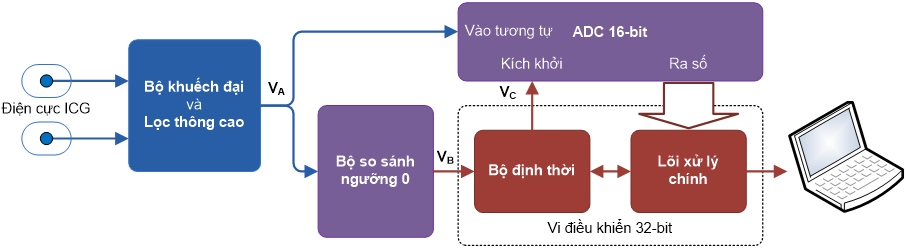
\includegraphics[width=16cm,height=4.39cm]{Images/hinh31.png}
    \caption[Sơ đồ khối của hệ thống]{\bfseries \fontsize{12pt}{0pt}\selectfont Sơ đồ khối của hệ thống}
    \label{hinh31}
\end{figure}
Hình \ref{hinh31} là ví dụ về cách chèn ảnh. Lưu ý chú thích của hình vẽ được đặt ngay dưới hình vẽ. Tất cả các hình vẽ phải được đề cập đến trong phần nội dung và phải được phân tích và bình luận giống như mình đang làm thế này nhé :)

\subsection{Cách tạo bảng}
\begin{table}[H]
    \centering
    \caption[Kết quả thí nghiệm]{\bfseries\fontsize{12pt}{0pt}\selectfont Kết quả thí nghiệm}
    \begin{tabularx}{0.85\textwidth}{
    | >{\centering\arraybackslash}y
    | >{\centering\arraybackslash}a
    | >{\centering\arraybackslash}a
    | >{\centering\arraybackslash}y|
    }
    \hline
    \bfseries  Lần thí nghiệm   &\bfseries Điện áp đo được \hspace{1cm}(mV)   &\bfseries Điện áp tham chiếu \hspace{0pt} (mV)  & \bfseries Sai lệch\hspace{0pt}(\%)\\\hline
       1  &   &   &\\\hline
       2  &   &   &\\\hline
       3  &   &   &\\\hline
    ...  &   &   &\\\hline
    \end{tabularx}
    \label{bang31}
\end{table}
Bảng \ref{bang31} là ví dụ về cách tạo bảng. Lưu ý chú thích của bảng được đặt ở trước bảng. Tất cả các bảng biểu phải được đề cập đến trong phần nội dung và phải được phân tích và bình luận giống như mình đang làm nhé :).

\subsection{Cách viết phương trình}
\begin{equation}\label{pt31}
    F(x) = \int^a_b \frac{1}{3}x^3
\end{equation}
Phương trình \ref{pt31} là ví dụ về phương trình tích phân.

Thử phương trình khác nhé :)
\begin{equation}\label{pt32}
    x[t_n] = \frac{1}{\sqrt{N}} \sum_{k=0}^{N-1}X[f_k]e^{j 2\pi n k/N}
\end{equation}
Phương trình \ref{pt32} thể hiện phép biến đổi Fourier rời rạc ngược (IDFT).

\subsection{Cách viết định nghĩa, định lý, hệ quả, bổ đề,...}
Định lý lấy mẫu Nyquist-Shannon là một định lý được sử dụng trong lĩnh vực lý thuyết thông tin, đặc biệt là trong viễn thông và xử lý tín hiệu.
\begin{theorem}\label{đlNq} % Định lý
Một hàm số tín hiệu $x(t_n)$ không chứa bất kỳ thành phần tần số nào lớn hơn hoặc bằng một giá trị $f_m$ có thể biểu diễn chính xác bằng tập các giá trị của nó với chu kỳ lấy mẫu $T=1/(2f_m)$.
\end{theorem}
Định lý \ref{đlNq} thường được gọi đơn giản là định lý lấy mẫu.
\begin{corollary}\label{coro1}
this is something here about corollary.
\end{corollary}
Hệ quả \ref{coro1} gì đó ....
\begin{lemma}\label{lemma1}
đây là nội dung bổ đề.
\end{lemma}
Bổ đề \ref{lemma1} ....
\begin{defn}\label{defn1}
Nội dung định nghĩa...
\end{defn}
Định nghĩa \ref{defn1} nói về...
\newpage
\section*{CHƯƠNG 4. THÍ NGHIỆM VÀ KẾT QUẢ}
\addcontentsline{toc}{section}{\numberline{}CHƯƠNG 4. THÍ NGHIỆM VÀ KẾT QUẢ}
\setcounter{section}{4}
\setcounter{figure}{0}
\setcounter{table}{0}
\lipsum
\begin{figure}[!ht]
    \centering
    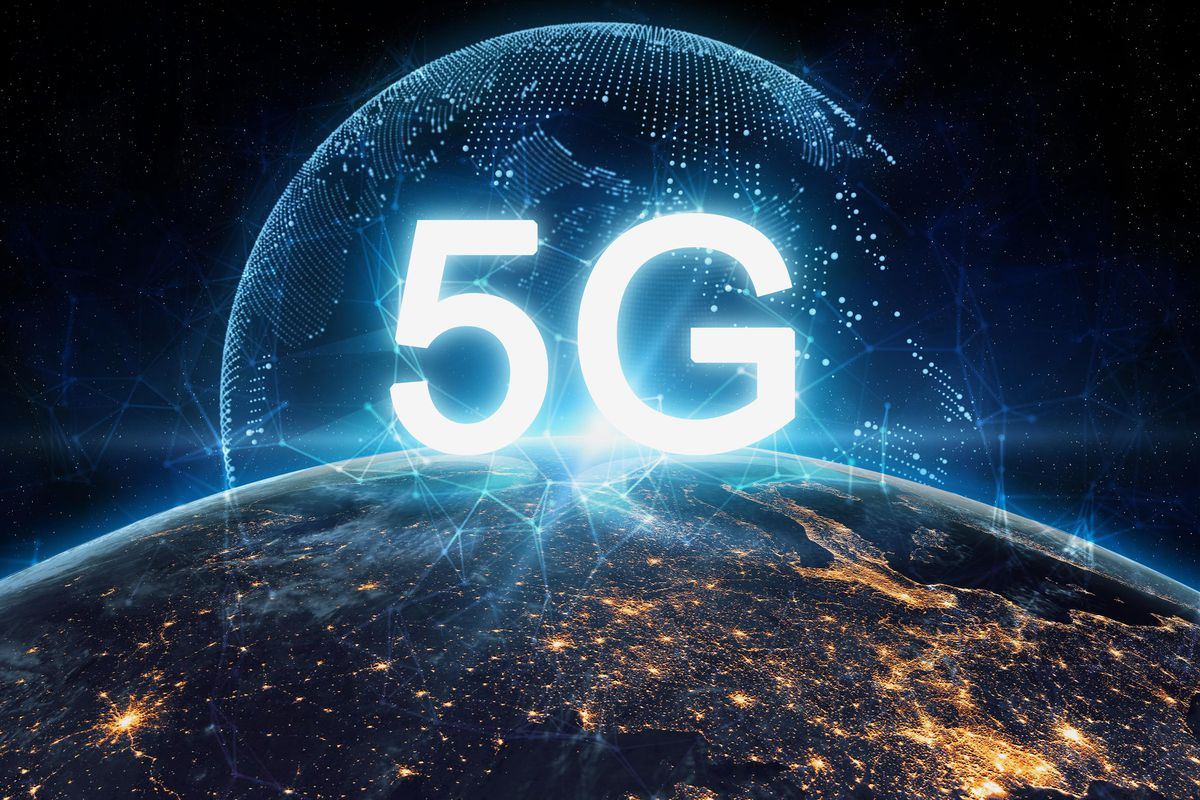
\includegraphics[width=16cm,height=6cm]{Images/5g.jpg}
    \caption[Mạng 5G]{\bfseries \fontsize{12pt}{0pt}\selectfont Mạng di động thế hệ thứ 5}
    \label{hinh41}
\end{figure}

Hình \ref{hinh41} là ví dụ về cách chèn ảnh. Lưu ý chú thích của hình vẽ được đặt ngay dưới hình vẽ. Tất cả các hình vẽ phải được đề cập đến trong phần nội dung và phải được phân tích và bình luận giống như mình đang làm thế này nhé :)
\newpage
\section*{KẾT LUẬN}
\phantomsection\addcontentsline{toc}{section}{\numberline {}KẾT LUẬN}
\subsection*{Kết luận chung}
\phantomsection\addcontentsline{toc}{section}{\numberline {}Kết luận chung}
Kết luận chung cho các chương trong đồ án. Mục này cần nhấn mạnh những vấn đề đã giải quyết và vấn đề chưa giải quyết để đưa ra các đánh giá về mức độ hoàn thành công việc. Đánh giá này thường bao gồm việc so sánh kết quả thu được với mục tiêu đề ra ban đầu.
\subsection*{Hướng phát triển}
\phantomsection\addcontentsline{toc}{section}{\numberline {}Hướng phát triển}
(Nếu có)
\subsection*{Kiến nghị và đề xuất}
\phantomsection\addcontentsline{toc}{section}{\numberline {}Kiến nghị và đề xuất}
(Nếu có)
\newpage
\phantomsection\addcontentsline{toc}{section}{\numberline {}TÀI LIỆU THAM KHẢO}
\bibliographystyle{IEEEtran}
\bibliography{TaiLieuThamKhao}
\newpage
\section*{PHỤ LỤC}
\phantomsection\addcontentsline{toc}{section}{\numberline{} PHỤ LỤC}
\texttt{
\fontsize{10pt}{0pt}\selectfont Mã nguồn chương trình (nếu có) được đưa vào đây, sử dụng font Courier New, cỡ 10pt.} % Phụ lục nếu có
\end{document}

